\chapter{Instalasi dan Konfigurasi Perangkat Lunak Prasyarat}\appcaption{Instalasi dan Konfigurasi Perangkat Lunak Prasyarat}

Pemasangan dan konfigurasi perangkat lunak adalah hal yang krusial. Sebelum dilakukan pemasangan perangkat lunak penyimpanan dan pemrosesan \textit{big data}, tentunya perlu disiapkan perangkat lunak prasyarat. Perangkat lunak prasyarat yang dibutuhkan meliputi Git, Java 8 dan Maven, Python 3.7, serta Scala 2.12. Langkah-langkah pemasangan dan konfigurasi perangkat lunak akan dijelaskan sebagai berikut,

\begin{enumerate}
  \item Pastikan Droplets pada DigitalOcean sudah dibuat. Masuk ke \textit{Virtual Machine} (VM) yang sebelumnya sudah dibuat melalui \textit{Console} yang berada pada laman konfigurasi Droplets DigitalOcean.
	\begin{center}
	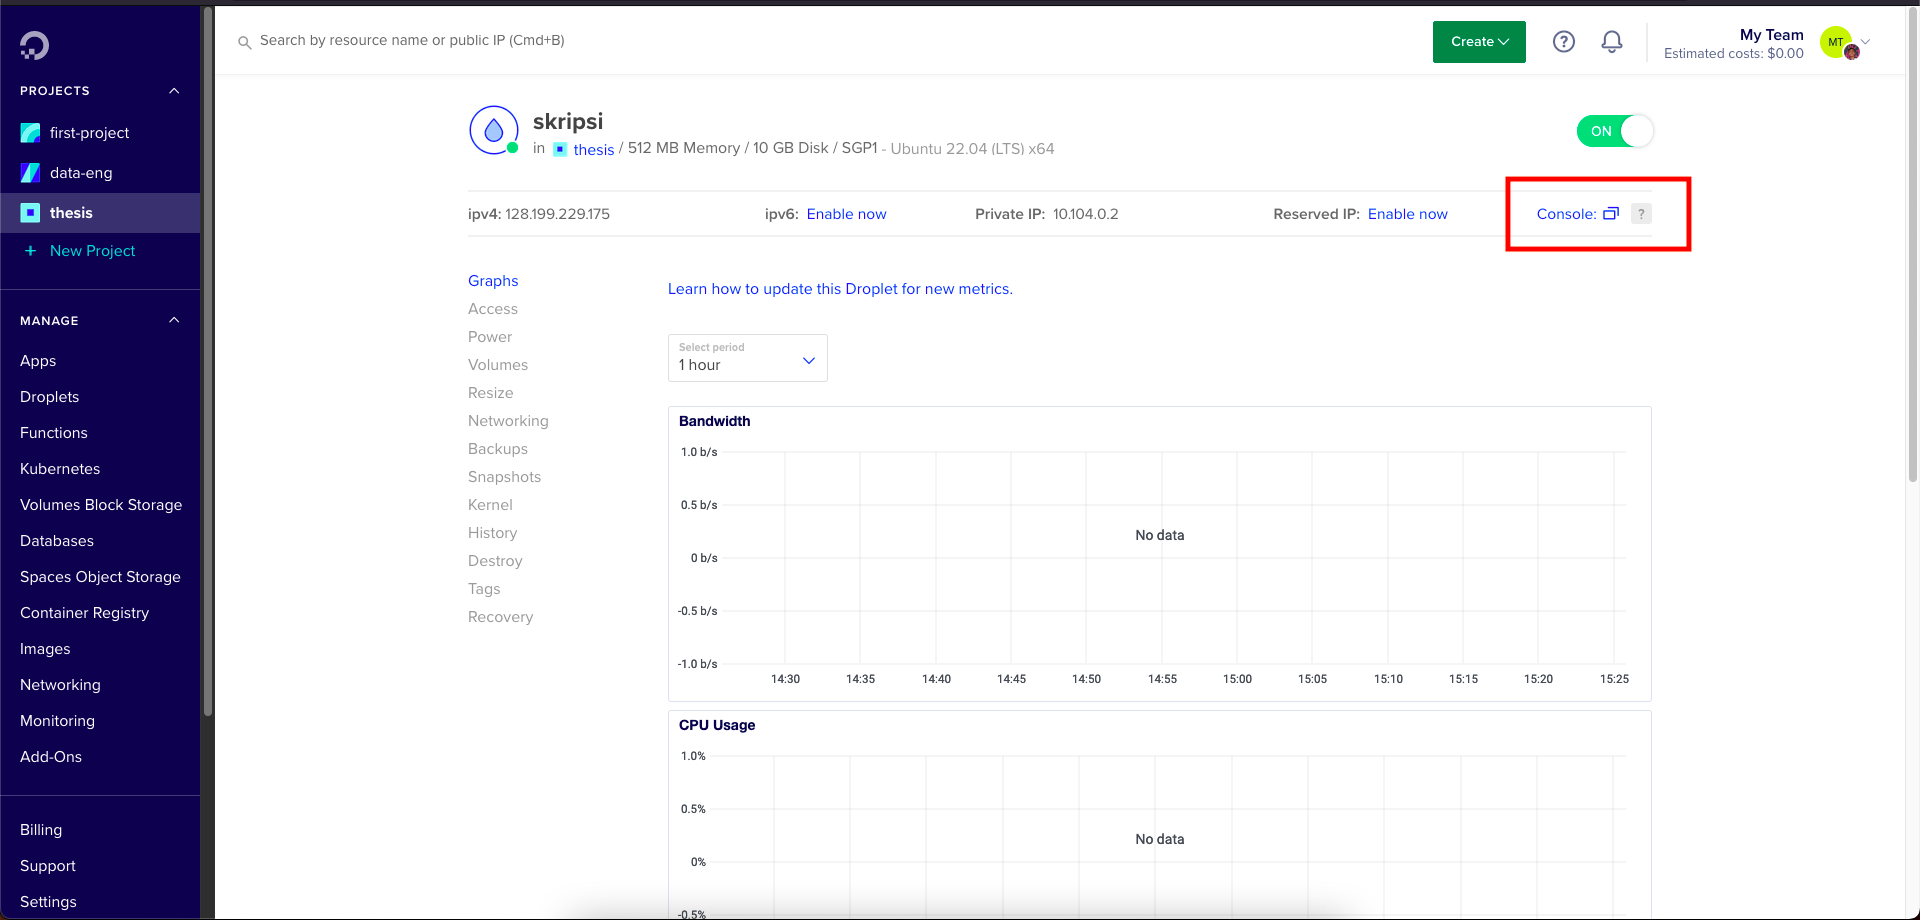
\includegraphics[width=1\linewidth]{figures/ch99/ap1/5.png}
	\end{center} 
  \item Jika Droplets baru saja dibuat, perlu dilakukan pembaruan \textit{index} pada \textit{package management}. \textit{Package management} adalah sistem atau sekumpulan alat yang digunakan untuk mengotomatiskan penginstalan, peningkatan, konfigurasi, dan penggunaan perangkat lunak. Pembaruan \textit{package management} dapat dilakukan dengan \verb|sudo apt update|. 
  \item Membuat Pengguna Baru   \begin{enumerate}
    \item Pertama, buatlah grup baru yang bernama \textit{hadoop} dengan perintah \verb|sudo addgroup hadoop|.
    \item Kemudian, tambahkan pengguna baru \textit{hdfsuser} dalam grup \textit{hadoop} yang sama dengan perintah \verb|sudo adduser --ingroup hadoop hdfsuser|.
    \item Berikan \textit{hdfsuser} izin \textit{root} yang diperlukan untuk pemasangan file. Hak istimewa pengguna \textit{root} dapat diberikan dengan memperbarui file \textit{sudoers}. Buka file \textit{sudoers} dengan menjalankan perintah \verb|sudo visudo|. Tambahkan baris berikut, yaitu \verb|hdfsuser ALL=(ALL:ALL) ALL|.
    \item Sekarang, simpan perubahan dan tutup editor.
    \item Selanjutnya, mari beralih ke pengguna baru yang telah dibuat untuk instalasi lebih lanjut menggunakan perintah \verb|su - hdfsuser|.
  \end{enumerate}
  \item Pengaturan \textit{SSH keys} untuk Hadoop
  \begin{enumerate}
  	\item Hadoop menggunakan \textit{Secure Shell} (SSH) untuk menjalankan proses antara \textit{master nodes} dan \textit{slave nodes}. Penggunaan SSH akan memberikan banyak keuntungan, salah satunya adalah kecepatan. Jika sebuah klaster aktif dan berjalan, komunikasi antar \textit{nodes} akan berjalan terlalu sering. Begitu pula dengan \textit{job tracker} yang harus sering mengirimkan informasi \textit{task to task} dengan cepat.Lakukan pemasangan ssh dan sshd dengan cara \verb|sudo apt-get install ssh| dan \verb|sudo apt-get install sshd| pada terminal.
    \item Selanjutnya, lakukan pembuatan \textit{SSH keys} dengan cara \verb|ssh-keygen -t rsa|. Jika pembuatan \textit{SSH keys} sudah dilakukan, jalankan perintah \verb|cat ~/.ssh/id_rsa.pub >> ~/.ssh/authorized_keys|.
    \item Ubah perizinan berkas dengan perintah \verb|chmod og-wx ~/.ssh/authorized_keys|.
    \item Terakhir, untuk memverifikasi koneksi aman sudah terjadi, lakukan \verb|ssh localhost|.
  \end{enumerate}
  \item Instalasi Git
  \begin{enumerate}
    \item Git dapat dipasang menggunakan perintah \verb|sudo apt install git|. Pengguna akan diminta konfirmasi untuk menginstall. Ketik \verb|y| kemudian tekan enter.
    \item Untuk mengecek versi Git, dapat menggunakan perintah \verb|git --version|.
  \end{enumerate}
  \item Instalasi Python 3.7
  \begin{enumerate}
    \item Python dapat dipasang menggunakan perintah \verb|sudo apt install python3.7|. Pengguna akan diminta konfirmasi untuk menginstall. Ketik \verb|y| kemudian tekan enter.
    \item Untuk mengecek versi Python, dapat menggunakan perintah \verb|python --version|.
  \end{enumerate}
  \item Instalasi Java 8 dan Maven
  \begin{enumerate}
    \item Java 8 dapat dipasang menggunakan perintah \verb|sudo apt install openjdk-8-jre-headless openjdk-8-jdk|. Pengguna akan diminta konfirmasi untuk menginstall. Ketik \verb|y| kemudian tekan enter.
    \item Versi dari Java dapat dilihat menggunakan perintah \verb|java -version|.
    \item Selanjutnya, instalasi Maven dapat dilakukan menggunakan perintah \verb| sudo apt-get -y install maven|.
    \item Informasi dari Maven beserta Java yang digunakan dapat dilihat menggunakan perintah \verb|mvn -version|.
  \end{enumerate}
  \item Instalasi Scala 2.12
  \begin{enumerate}
    \item Scala yang akan dipasang adalah versi 2.12. Jika menggunakan manajer paket, versi yang akan dipasang adalah versi terbaru. Untuk mengunduh versi spesifik dari Scala, dapat menggunakan perintah \verb|sudo apt install wget|, dilanjutkan dengan \verb|sudo wget  https://downloads.lightbend.com/scala/| \verb|2.12.18/scala-2.12.18.deb|.
    \item Scala dapat dipasang menggunakan perintah \verb|sudo dpkg -i scala-2.12.18.deb|.
    \item Versi Scala dapat dilihat melalui perintah \verb|scala -version|.
  \end{enumerate}
\end{enumerate}